\chapter{Asking Millionaires How They Got RICH! (Dallas)}

This chapter is built from a street-level lecture on wealth rather than from a blackboard derivation. The host walks Highland Park in Dallas, encounters executives, owners, and athletes, and keeps asking the same family of questions: how was scale built, what actually mattered, and what should a younger entrepreneur imitate? If we keep the lecture in its spoken order, a real structure appears. We move from spectacle to mechanism, from visible wealth to the operating rules beneath it, and finally from acquisition to stewardship.

\section{Dallas as a Field Test for Wealth}

The lecture opens with a teaser reel of cars, titles, and income fragments. We should not read that opening as chronology. It is a montage borrowing from later moments in the lecture in order to set the tone. Only after that burst of spectacle does the host stabilize the setting: Highland Park is presented as the wealthiest area in Dallas, and Dallas itself is framed by the host as a city dense with millionaires. The method is then fixed. We will ask people in public how they became successful.

The recurring question is simple enough that it behaves almost like an operator acting on different domains:
\[
\text{visible success} \longmapsto \text{extractable mechanism}.
\]
That is the lecture's central move. It begins with a Rolls-Royce, a title, or a number, and then immediately asks for the structure beneath the surface.

Because the cold open intercuts later material, the first quantitative ledger is deliberately non-chronological. It tells us what kinds of scale the lecture will eventually organize into cases:

\begin{align}
I_{\mathrm{peak}} &\in \{\text{multiple seven figures},\ \ \$11\text{ million}\},\\
R_{\mathrm{biz}} &\approx \$60\text{ million},\\
V_{\mathrm{ops}} &\approx \$700\text{ million},\\
V_{\mathrm{exit}} &\in \{\$365\text{ million},\ \ \$3.5\text{ billion}\},\\
N_{\mathrm{loc}} &\ge 75,\qquad N_{\mathrm{states}} = 13.
\end{align}

Nothing here is yet a theory. The lecture begins, rather, by showing us that the sample is nontrivial: athletes with eight-figure years, operators running nine-figure businesses, owners with multi-state footprints, and executives involved in very large exits. Once that is established, the lecture starts turning these scales into rules.

\section{Consumer Obsession and Character at Scale}

The first major doctrinal statement comes from the Frito-Lay CEO. The host is visibly surprised by the discovery, and that surprise is part of the pedagogy. The lecture wants us to feel the jump from ordinary street encounter to genuine operator. Only then does it ask the sharper question: what does it take to build something on that scale?

The answer is given in two layers. First there is the founding myth: Herman Lay selling potato chips from a truck, hustling, doing things the right way, taking care of customers, taking care of employees. Then there is the update for the present day: understand the consumer better than anybody else, watch trends through technology, and remain consumer-obsessed.

A compact way to record the lecture's order is
\begin{equation}
\text{founder hustle}
\longrightarrow
\text{customer care and employee care}
\longrightarrow
\text{consumer understanding with technological feedback}
\longrightarrow
\text{scale}.
\end{equation}

This is not a quantitative law. It is a map of emphasis. The lecture first keeps open the possibility that a giant firm can begin from one person's effort. It then immediately corrects any naive reading of that myth by insisting that modern scale depends on knowing the consumer in real time.

When the host presses further and asks what enabled the rise to chief executive rank, the answer again refuses a single magic variable. Preparation matters. Luck matters. Being in the right place at the right time matters. But the moral claim arrives at once: if one works hard and is brilliant but treats people badly, the whole thing can still fail. The lecture is already moving away from solitary heroics and toward social machinery.

\section{The Company Is Not the CEO}

The next interview shifts the lecture from founder mythology to organizational design. The speaker, who ran major retail companies including JCPenney, Macy's, Barneys, and Neiman Marcus, states the thesis with unusual bluntness: the CEO does not make the company successful by himself. The people who work for the company do that. The CEO's responsibility is to make those people understand how important they are.

This is more than a moral gesture. It becomes a structural claim about how large firms work. Different companies have different cultures, and the leader must first understand who the company is, not merely impose who he is. The argument then sharpens into a hierarchy of causation.

\begin{proposition}
In the lecture's management logic, shareholder welfare is downstream of culture, customer understanding, and the treatment of employees.
\begin{equation}
\text{culture}
\longrightarrow
\text{customer care} + \text{employee care}
\longrightarrow
\text{shareholder outcome}.
\end{equation}
\end{proposition}

\begin{proof}
The speaker grants that the shareholder formally comes first in one sense: the shareholder can fire management. But the lecture's practical claim is that management cannot reach the shareholder through direct loyalty to the shareholder alone. If the customer is neglected, the firm loses its market. If employees are neglected, the firm loses execution. In either case, shareholder value deteriorates. Thus the route to the shareholder is indirect and operational.
\end{proof}

The host then asks for a blueprint for building a strong company in the present environment, and the answer preserves the same order: understand culture, understand the customer, take care of the people, and only then do we arrive at a durable company.

\subsection{Question \& Answer}

\paragraph{Question.} If shareholders formally come first, what should management actually put first in practice?

\paragraph{Answer.} The lecture answers by separating formal hierarchy from causal hierarchy. We begin with the culture of the company, then with the customer, then with the treatment of employees. Only through that chain do we reach the shareholder in a durable way. This is one of the lecture's central reversals, and it should not be flattened into generic ``stakeholder'' language; the point is specifically that the path to shareholder value runs through the rest of the organization.

\section{Discipline, Exits, and the Move from Earnings to Capital}

The lecture next broadens the sample by moving from corporate executives to Tavon Austin. This matters for the narrative. We are no longer talking about a chief executive, yet the structure of the answer is strikingly familiar. Success is again presented as a bundle rather than a single talent: discipline, hard work, focus, the desire to escape a limiting environment, and the refusal to surround oneself with yes-men.

The athlete segment also gives the lecture a clean money marker. Tavon Austin states that his biggest single-year income was about \$11 million. But the financial lesson attached to that figure is not extravagance. It is the need for financial advisors and trusted people who will act as a backbone and say no when necessary. So even here, at the point where the lecture could become pure earnings spectacle, it turns instead toward constraint and guardrails.

From there we move into a healthcare entrepreneur's account, and the lecture changes gears from earnings to exits. The speaker explains that his graduate degree was in public administration, but that his business life moved into oncology and clinical trials. The business scale is stated at about \$60 million, while an earlier company had been sold for about \$365 million. The speaker is careful to note that the sale was not a solitary triumph: ``there was a group of us.'' The host then pauses and converts that into doctrine. Large wealth, in this lecture, is repeatedly a team-made event.

That shift from earnings to capital then becomes a shift from capital to sector choice. The speaker's financial advice is to invest early and not too late, and his sector claim is concrete enough to preserve. Oncology, he says, has changed materially over the last couple of decades.

\begin{equation}
D_{\mathrm{onc}}(t_0) \approx 12\text{--}15,
\qquad
D_{\mathrm{onc}}(t_1) > 40.
\end{equation}

Here \(D_{\mathrm{onc}}(t)\) denotes, in the loose language of the lecture, the number of ``good'' oncology drugs available at a given time. This is not a formal biomedical metric, and we should not pretend otherwise. But it does give the lecture a factual spine: the speaker's argument for healthcare, and especially for drug development, is that the technical base of the field has widened, with immune therapy named as one major reason.

At this stage of the lecture we can already see the progression: first earn, then build, then exit, then reinvest where technical progress is making new bets intelligible.

\section{Delegation and the Arithmetic of Scaled Ownership}

The tanning-franchise owner gives the lecture its clearest machinery. The footprint is large, the income is large, but the real interest is in the explanation of how ownership scales beyond the labor of the owner. The first obstacle named is control. People want to touch everything themselves. The speaker's answer is a delegation threshold.

\begin{definition}
Delegation, in the sense used in this lecture, means handing off a task when another operator can perform it at roughly seventy percent of the owner's level, provided the release of owner attention creates more value than the loss of direct control.
\end{definition}

The threshold may be written schematically as
\begin{equation}
q_{\mathrm{delegate}} \ge 0.7\,q_{\mathrm{owner}}.
\end{equation}

We should read this with caution. It is a spoken managerial heuristic, not an optimization theorem. Nevertheless it is mathematically useful because it preserves the speaker's real point: insisting on personal perfection blocks scale, while accepting good-enough execution multiplies reach.

The second mechanism is equity. The owner says he will buy a company, give somebody equity, let that person treat it as their baby, and allow them to do most of the work while he supplies structure, books, team, and resources. This is the chapter's clearest case of ownership income being separated from direct daily execution.

\paragraph{Worked example.} The lecture gives a numerical case precise enough to compute. A business earns \$600{,}000 in profit and is owned by two equal partners. Then
\begin{align}
P_{\mathrm{biz}} &= \$600{,}000,\\
\alpha &= \tfrac12,\\
\alpha P_{\mathrm{biz}} &= \tfrac12 \cdot \$600{,}000 = \$300{,}000.
\end{align}

The arithmetic is elementary, but we should preserve the logic step by step:

\begin{enumerate}
\item Take the stated business profit \(P_{\mathrm{biz}}=\$600{,}000\).
\item Impose equal ownership, so \(\alpha=\tfrac12\).
\item Compute one partner's share as \(\alpha P_{\mathrm{biz}}\).
\item Obtain \(\$300{,}000\) for each side.
\item Interpret the result as structured ownership income rather than as income from direct daily execution.
\end{enumerate}

The lecture also adds an important correction: there is ``no such thing as passive income'' in a fully literal sense. What we have instead is an arrangement in which someone else performs most of the operating labor while ownership, capital, and systems capture part of the outcome. That is not metaphysical passivity; it is organizational leverage.

\section{Concentration, Diversification, and Vertical Integration}

Once the lecture has explained how an owner can step back from direct labor, it raises the next strategic question. Should the entrepreneur diversify early, or concentrate?

The answer is given in a slogan because the slogan is genuinely useful:
\begin{equation}
\mathrm{Concentration} \longrightarrow W,
\qquad
\mathrm{Diversification} \longrightarrow \mathrm{preserve}(W).
\end{equation}
Here \(W\) denotes accumulated wealth or, more practically, a durable cash-flow base.

The lecture's order matters. We first concentrate on one thing until it becomes serious enough to replace the day job and generate discretionary power. Only then do we diversify. That is why the owner mocks the thin version of the ``multiple streams of income'' idea: two tiny streams do not yet solve the scale problem.

\subsection{Question \& Answer}

\paragraph{Question.} Should the entrepreneur begin by building many small income streams?

\paragraph{Answer.} The lecture says no. Early diversification is usually a way of avoiding concentration rather than a way of building wealth. We first scale one thing until it throws off serious cash flow. Only then do we move sideways into preserving or adjacent assets. Diversification is stage two, not stage one.

The lecture then sharpens the point by distinguishing random diversification from vertical integration. The owner says that he is opening about twenty new locations and is spending on the order of \$200{,}000 in one month just on HVAC. That spending suggests a direction:

\begin{equation}
N_{\mathrm{new}} = 20,
\qquad
C_{\mathrm{HVAC,month}} \approx \$200{,}000.
\end{equation}

If the operating business repeatedly pays outside firms for HVAC, electrical work, plumbing, architecture, commissions, and real estate, one can acquire or control some of those adjacent channels and internalize the margin. The speaker's cleanest example is rent: if the business occupies buildings that the owner also owns, rent is being paid to oneself.

We can record the resulting logic schematically as
\begin{equation}
\Pi_{\mathrm{integrated}}
=
\Pi_{\mathrm{core}}
+
\Pi_{\mathrm{HVAC}}
+
\Pi_{\mathrm{electrical}}
+
\Pi_{\mathrm{plumbing}}
+
\Pi_{\mathrm{arch}}
+
\Pi_{\mathrm{real\ estate}}.
\end{equation}

This is not an accounting identity from the lecture. It is a careful reconstruction of the speaker's mechanism: external cost centers can be turned into internal profit streams.

\begin{figure}
\centering
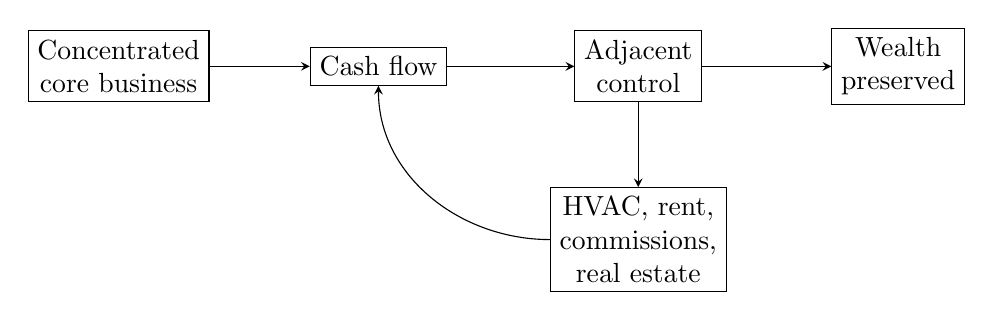
\begin{tikzpicture}[>=stealth]
\node[draw, rectangle, align=center] (a) at (0,0) {Concentrated\\core business};
\node[draw, rectangle, align=center] (b) at (3.3,0) {Cash flow};
\node[draw, rectangle, align=center] (c) at (6.6,0) {Adjacent\\control};
\node[draw, rectangle, align=center] (d) at (9.9,0) {Wealth\\preserved};
\node[draw, rectangle, align=center] (e) at (6.6,-2.2) {HVAC, rent,\\commissions,\\real estate};

\draw[->] (a) -- (b);
\draw[->] (b) -- (c);
\draw[->] (c) -- (d);
\draw[->] (c) -- (e);
\draw[->] (e.west) to[out=180,in=-90] (b.south);
\end{tikzpicture}
\end{figure}

The figure is editorial rather than documentary, but it is faithful to the sequence of the lecture. We begin with concentration. Concentration gives cash flow. Cash flow permits control over adjacent channels. That control feeds margin back into the same system and turns diversification from distraction into preservation.

\section{Peace, Dry Powder, and the Tipping Point}

Before the lecture turns to the final executive interview, it interrupts itself with a short but important correction. Dante says, in essence, that peace should be sought instead of financial gain. The host immediately translates this into the lecture's vocabulary: if we pursue money alone, we do not arrive at peace or happiness. This interruption is brief, but structurally it matters. It forces the lecture to distinguish the accumulation of wealth from the orientation of the person accumulating it.

The final interview then returns to a more formal business register. We are back in healthcare, now with a former chief operating officer of a \$700 million business that was sold to private equity for about \$3.5 billion at the end of 2020. The first major object introduced here is liquidity.

\begin{definition}
Dry powder is liquid cash held in reserve so that one can respond to opportunities, people, ideas, and obligations when they appear.
\end{definition}

The lecture's practical rule is
\begin{equation}
E \approx \tfrac12 I,
\qquad
C_{\mathrm{dry}} = I - E > 0,
\end{equation}
where \(I\) is income, \(E\) is spending, and \(C_{\mathrm{dry}}\) is the reserve held on the sideline. The advice is approximate, not exact. The point is not that half is sacred. The point is that if liquidity is driven to zero, optionality is destroyed.

The lecture next asks what carries a business from seven figures to eight and nine. The answer is not a single trick but a list of infrastructure components: people, technology, sales, marketing, and commercialization. These are assembled until the product becomes what the speaker calls an industry utility, that is, something whose absence creates a disadvantage.

We can preserve the causal chain as
\begin{equation}
K_{\mathrm{scale}}
=
K_{\mathrm{people}}
+
K_{\mathrm{tech}}
+
K_{\mathrm{sales}}
+
K_{\mathrm{marketing}}
+
K_{\mathrm{comm}}
\longrightarrow
U_{\mathrm{industry}}.
\end{equation}

Again, this is schematic rather than measured. But it keeps the lecture's logic in place. Scale is not merely a larger idea. It is a larger apparatus.

The last answer of the lecture closes the chapter cleanly. What most drove the executive's rise was helping others succeed. One hires strong people, mentors them, pulls them up, gives them criticism that is usable, and thereby creates a system in which one's own rise is tied to the rise of others. At the end of the lecture, the strongest general principle is no longer private genius. It is structured cooperation.

\section{Summary}

If we flatten this lecture, we get a stack of millionaire anecdotes. If we preserve its rhythm, we get something more useful. The host begins with wealth-signals, then keeps converting those signals into mechanisms. Consumer businesses scale through customer knowledge and technological attention. Large firms are not made by the CEO alone, but by culture, customers, and employees. Athletes need discipline and financial guardrails. Entrepreneurs can turn earnings into capital through exits and reinvestment. Owners scale through delegation and equity. Concentration should generally precede diversification, while vertical integration converts external margins into internal ones. Peace cannot be replaced by money, liquidity preserves optionality, infrastructure creates tipping points, and the most durable route upward is to help capable people rise with us.

The mathematics is light, but it is real. The lecture gives us thresholds, counts, splits, reserves, and causal chains. That is enough to turn street interviews into a serious companion text on wealth-building: not a mythology of success, but a sequence of concrete mechanisms by which scale is built, protected, and made livable.